\documentclass[10pt,a4paper]{article}
\usepackage[utf8]{inputenc}
\usepackage[italian]{babel}
\usepackage{amsmath}
\usepackage{amsfonts}
\usepackage{amssymb}
\usepackage{graphicx}
\usepackage{siunitx}
\usepackage[left=2cm,right=2cm,top=2cm,bottom=2cm]{geometry}
\newcommand{\rem}[1]{[\emph{#1}]}
\newcommand{\exn}{\phantom{xxx}}

\author{Gruppo 1.BN \\ Massimo Bilancioni, Alessandro Foligno, Giuseppe Zanichelli }
\title{Amplificatore a transistor}


\begin{document}

\date{4 ottobre 2018}
\maketitle

\section{Risposta a segnali sinusoidali di frequenza fissa}

Abbiamo scelto una frequenza di lavoro intorno ai $7.40$ \si{\kilo\hertz}.

a) 
\vspace{0.5cm}
i)  Abbiamo verificato l'inversione di fase per VOUT rispetto a VIN

\begin{figure}[h]
	\centering
	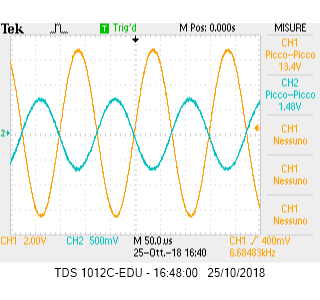
\includegraphics[scale=0.5]{oscilloscopio.png}

	
	
\end{figure}

ii)
\begin{table}[h]
	\centering
	\begin{tabular}{|c|c|c|}
		\hline 
		 VIN (\si{\volt}) &  VOUT (\si{\volt})   & VOUT/VIN\\
		\hline 
	0.228 & 2.20& 9.65 \\
	0.320 & 3.12 & 9.75 \\
	0.528 & 5.14 & 9.73 \\
	0.752& 7.32 & 9.73\\
	1.02 & 10.2& 10 \\
	1.27& 12.3 & 9.69 \\
		\hline 
	\end{tabular} 
\end{table}

iii) Per un segnale in ingresso di circa $1.60$ \si{\volt}pp si iniziano a vedere distorsioni per VOUT.

iv)\begin{figure}[h]
	\centering
	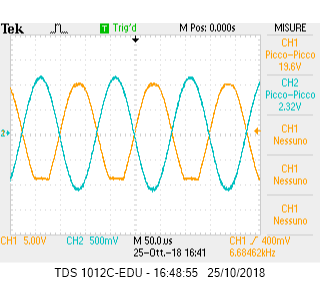
\includegraphics[scale=0.5]{clipping.png}

	
	
\end{figure}

	

\section*{Dichiarazione}
I firmatari di questa relazione dichiarano che il contenuto della relazione \`e originale, con misure effettuate dai membri del gruppo, e che tutti i firmatari hanno contribuito alla elaborazione della relazione stessa.

\end{document}